\chapter{Lecture 7: ....}\label{lec:7}
\begin{center}
  {\LARGE\bfseries\color{aaublue}
    MM7 subsection Networks and Systems}\\[0.4em]
  {\large\color{accentgray}
    Topic Notes: Performance Implications of Data Access Schemes}\\[0.2em]
  {\large\bfseries Slides 1--11}\\[0.3em]
  {\small\color{accentgray}
    Hans-Peter Schwefel, Aalborg University}
\end{center}


% ============================================================
\section{The Wind Farm Scenario (Slides 2--3)}
% ============================================================
\begin{figure}[H]
    \centering
    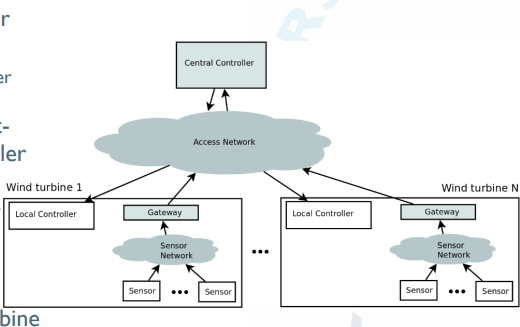
\includegraphics[width=0.7\linewidth]{figures/Lecture7/windfarmscenerio.png}
    \label{fig:placeholder}
\end{figure}
The lecture is motivated by a real engineering problem: a \textbf{central
controller} must manage multiple wind turbines remotely. The objective is to
minimise mechanical \textbf{damage} to the turbines while maintaining a target
power output.
 
To achieve this, the controller needs \textbf{fresh sensor data} from each
turbine (torque $\times 2$, rotation angle --- 3 sensors per turbine). This
data must travel over a network that introduces \textbf{delay}, meaning the
controller may act on \emph{stale} information.
 
\subsection{System Architecture}
 
The communication architecture has two layers:
 
\begin{itemize}[leftmargin=2em]
  \item \textbf{Sensor Network} (e.g.\ CANbus, Fieldbus) --- sensors
        communicate with a local gateway at each turbine.
  \item \textbf{Access Network} (e.g.\ LTE, 3G, fiber, PLC) --- the gateway
        relays data to the central controller.
\end{itemize}
 
Key timing constraint: the controller acts every $T_s = 150\,\text{ms}$, so
data freshness is critical.
 
\begin{insightbox}
\textbf{Central tension:} How should sensors deliver data to the controller,
and what are the performance consequences of each approach?
\end{insightbox}
 
% ============================================================
\section{Different Access Strategies (Slide 4)}
% ============================================================
 \begin{figure}[H]
     \centering
     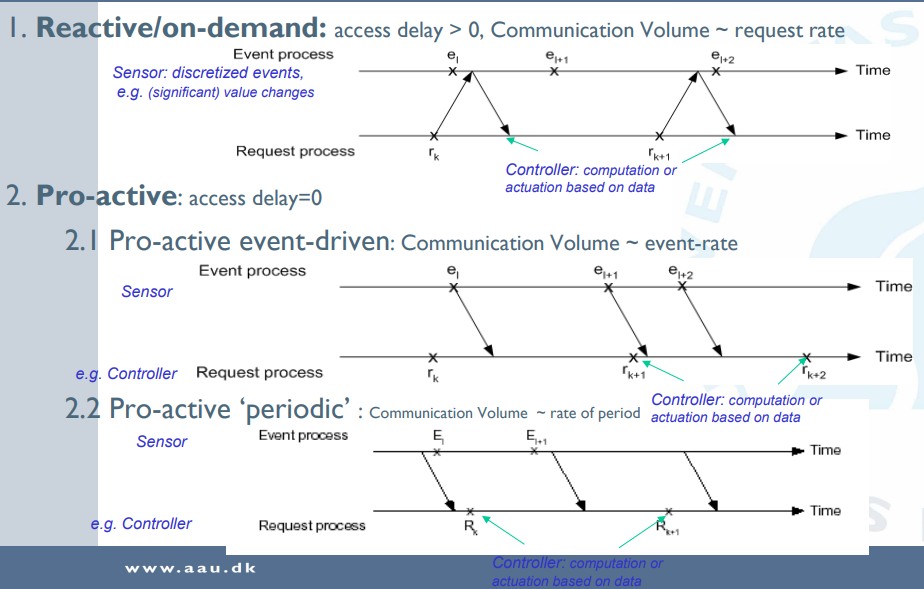
\includegraphics[width=\linewidth]{figures/Lecture7/accessStragies.png}
     \label{fig:placeholder}
 \end{figure}
There are two fundamental philosophies for data delivery:
 
\subsection{1.\ Reactive (On-Demand / Pull)}
 
The controller \emph{requests} data when it needs it; the sensor responds.
 
\begin{itemize}[leftmargin=2em]
  \item Access delay $> 0$ (round-trip: request upstream + data downstream).
  \item Communication volume $\sim$ request rate.
\end{itemize}
 
\subsection{2.\ Proactive (Push)}
 
The sensor sends data \emph{without being asked}; access delay $= 0$ because
the controller already holds the latest value. This splits into two sub-types:
 
\subsubsection*{2.1 \ Proactive Event-Driven}
An update is sent whenever a \emph{significant change} occurs at the sensor.
\begin{itemize}[leftmargin=2em]
  \item Communication volume $\sim$ event rate.
\end{itemize}
 
\subsubsection*{2.2 \ Proactive Periodic}
Updates are sent on a fixed clock, regardless of whether anything has changed.
\begin{itemize}[leftmargin=2em]
  \item Communication volume $\sim$ period rate.
\end{itemize}
 
\begin{insightbox}
The slide 4 timing diagrams illustrate the misalignment between sensor events
and controller requests in the reactive case, and how proactive strategies
eliminate this waiting gap.
\end{insightbox}
 
% ============================================================
\section{Taxonomy of Cases (Slide 5)}
% ============================================================
 
Slide 5 extends the classification into a decision tree. After choosing
reactive or proactive, further choices arise:
 
\begin{itemize}[leftmargin=2em]
  \item \textbf{Full updates vs.\ incremental updates} --- does each message
        carry the complete current value, or only the \emph{change} since last
        time?
  \item \textbf{Message ordering} --- by sender sequence number (SEQno) or by
        receive time? This matters because network packets can arrive out of
        order.
\end{itemize}
 
The circled nodes in the tree on slide 5 are the specific cases analysed
mathematically later in the lecture.
 \begin{figure}[H]
     \centering
     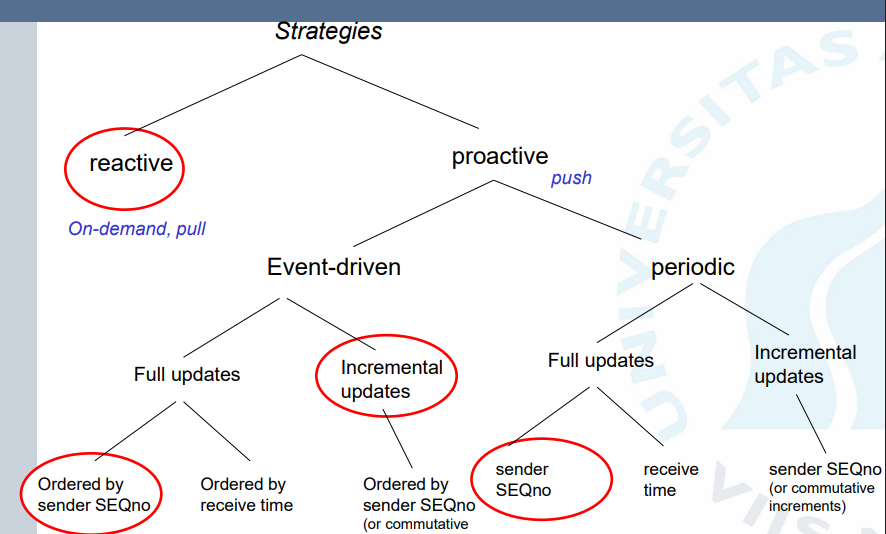
\includegraphics[width=0.8\linewidth]{figures/Lecture7/tree.png}
     \label{fig:placeholder}
 \end{figure}
% ============================================================
\section{Performance Metric: Mismatch Probability (Slide 6)}
% ============================================================
 
To compare all strategies on a common footing the lecture defines the
\textbf{mismatch probability} $\mathrm{mmPr}$:
 
\begin{mdframed}[backgroundcolor=lightgray, linecolor=aaublue, linewidth=1.5pt,
  leftline=true, rightline=false, topline=false, bottomline=false,
  innerleftmargin=10pt, innertopmargin=6pt, innerbottommargin=6pt]
$\mathrm{mmPr}$ = probability that the value the controller \emph{believes}
the sensor has does \textbf{not} match the sensor's \emph{actual} value at the
instant the controller uses the information.
\end{mdframed}
 
\subsection{Participating Processes}
 
Five stochastic processes are identified:
 
\begin{enumerate}[leftmargin=2em]
  \item \textbf{Event process} $\mathcal{E}$ (Poisson, rate $\lambda$) ---
        significant value change at the sensor.
  \item \textbf{Request process} $\mathcal{R}$ (rate $\mu$) --- controller
        requests sensor information.
  \item \textbf{Downstream delay} $\mathcal{D}$ (Poisson, rate $\nu$) ---
        propagation from sensor to controller.
  \item \textbf{Upstream delay} $U$ --- propagation from controller to sensor
        (reactive case only).
  \item \textbf{Period} $\mathcal{P}$ (Poisson, rate $\tau$) --- update
        interval for proactive periodic strategy.
\end{enumerate}
 
\subsection{Key Assumptions}
 
\begin{itemize}[leftmargin=2em]
  \item All processes are mutually independent $\Rightarrow$ the request
        process is irrelevant for the stationary $\mathrm{mmPr}$.
  \item Messages may be reordered in the network, but the receiver can restore
        order using sequence numbers.
  \item The information element \emph{never reverts} to an earlier value
        (monotone behaviour assumed).
\end{itemize}
 
% ============================================================
\section{Analysis of Each Strategy (Slides 7--9)}
% ============================================================
 
\subsection{Reactive Case (Slide 7)}
 
Let $A(t)$ be the CDF of the \emph{forward recurrence time} of the Poisson
event process (i.e.\ the remaining time until the next event, seen from an
arbitrary point in time). For a Poisson process with rate $\lambda$:
$A(t) = 1 - e^{-\lambda t}$.
 
The mismatch probability is:
\begin{align}
  \mathrm{mmPr}
    &= 1 - \int_{t=0}^{\infty} \bigl(1 - A(t)\bigr)\, f_D(t)\, dt \notag \\
    &= 1 - \int_{0}^{\infty} e^{-\lambda t}\, f_D(t)\, dt \notag \\
    &= 1 - \mathcal{L}\{f_D\}(\lambda),
\end{align}
where $\mathcal{L}\{f_D\}(\lambda)$ is the Laplace transform of the delay PDF
evaluated at the event rate $\lambda$.
 
\begin{insightbox}
\textbf{Intuition:} if the network is fast ($D$ small) relative to how often
values change ($\lambda$ large), mismatches are rare. A faster network
directly improves data freshness.
\end{insightbox}
 \begin{figure}[H]
    \centering
    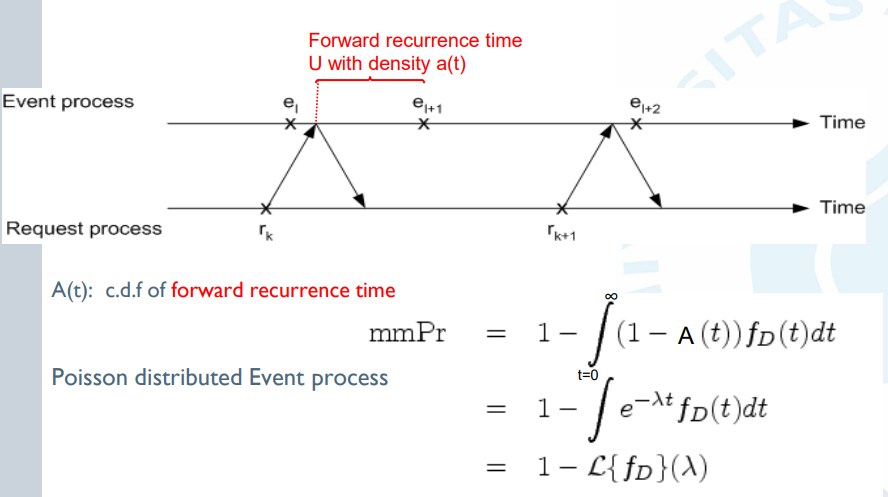
\includegraphics[width=\linewidth]{figures/Lecture7/reactiveanal.png}
    \label{fig:placeholder}
\end{figure}
\subsection{Proactive Event-Driven Case (Slide 8)}
 
Two sub-cases arise depending on the update type.
 
\subsubsection*{(a) Incremental Updates}
 
A mismatch occurs only if a message is \emph{still in transit} when the
controller acts. This is equivalent to asking whether an
$\mathcal{E}/\mathcal{D}/\infty$ queue is busy:
\begin{equation}
  \mathrm{mmPr} = \Pr\!\left(\text{M/M}/\infty \text{ queue is busy}\right)
               = 1 - e^{-\lambda/\nu}.
\end{equation}
This result is \textbf{independent of the delay distribution} --- only the
ratio $\lambda/\nu$ matters.
 
\subsubsection*{(b) Full Updates}
 
A mismatch occurs if the \emph{last} message sent is still in transit:
\begin{align}
  \mathrm{mmPr}_{\text{proact,full}}
    &= 1 - \int_{0}^{\infty} P(\mathcal{D} \leq t \mid U = t)\, a(t)\, dt
     \notag \\
    &= 1 - \int_{0}^{\infty} P(\mathcal{D} \leq t)\, a(t)\, dt,
\end{align}
where $a(t)$ is the density of the \emph{backward recurrence time} of the
event process. This is \textbf{identical to the reactive case} --- a
surprising result.
\begin{figure}[H]
    \centering
    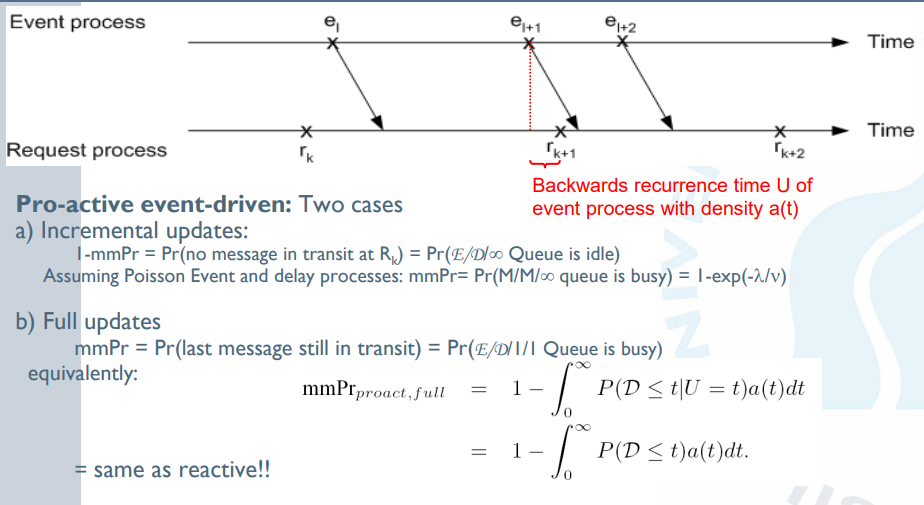
\includegraphics[width=\linewidth]{figures/Lecture7/eventdrivenanal.png}
    \label{fig:placeholder}
\end{figure}
\subsection{Proactive Periodic Case (Slide 9)}
 
This is the most complex case, modelled as a \textbf{continuous-time Markov
chain} whose second state component counts the number of useful messages
currently in transit.
 
The stationary matching probability $\pi_1 = 1 - \mathrm{mmPr}$ has the
explicit solution:
\begin{equation}
  \pi_1 = \frac{
    \dfrac{\nu}{\lambda}
    \displaystyle\sum_{n=3}^{\infty}(n-2)
      \prod_{i=1}^{n-2}\dfrac{\tau}{i\nu+\tau+\lambda}
  }{
    1 + \dfrac{\nu}{\lambda}
    \displaystyle\sum_{n=3}^{\infty}(n-1)
      \prod_{i=1}^{n-2}\dfrac{\tau}{i\nu+\tau+\lambda}
  }.
\end{equation}
 
An alternative closed-form representation using the gamma distribution CDF is:
\begin{equation}
  \mathrm{mmPr} = \frac{\lambda}{\nu}
    \exp\!\left(\frac{\tau}{\nu}\right)
    \frac{
      \Gamma\!\left(\dfrac{\tau+\lambda}{\nu}\right)
    }{
      \left(\dfrac{\tau}{\nu}\right)^{(\tau+\lambda)/\nu}
    }
    F_{\Gamma\!\left(\frac{\tau+\lambda}{\nu},\,\frac{\tau}{\nu}\right)}(1).
\end{equation}
 
\begin{insightbox}
\textbf{Key insight (large $\nu$ limit):} even with a perfect (infinitely
fast) network, the periodic strategy has a fundamental accuracy floor:
\[
  \mathrm{mmPr} \;\xrightarrow{\nu\to\infty}\; \frac{\lambda}{\lambda+\tau}.
\]
No amount of network improvement can push $\mathrm{mmPr}$ below this ceiling
--- it is set entirely by how often updates are sent ($\tau$) relative to how
often the value changes ($\lambda$).
\end{insightbox}
\begin{figure}[H]
    \centering
    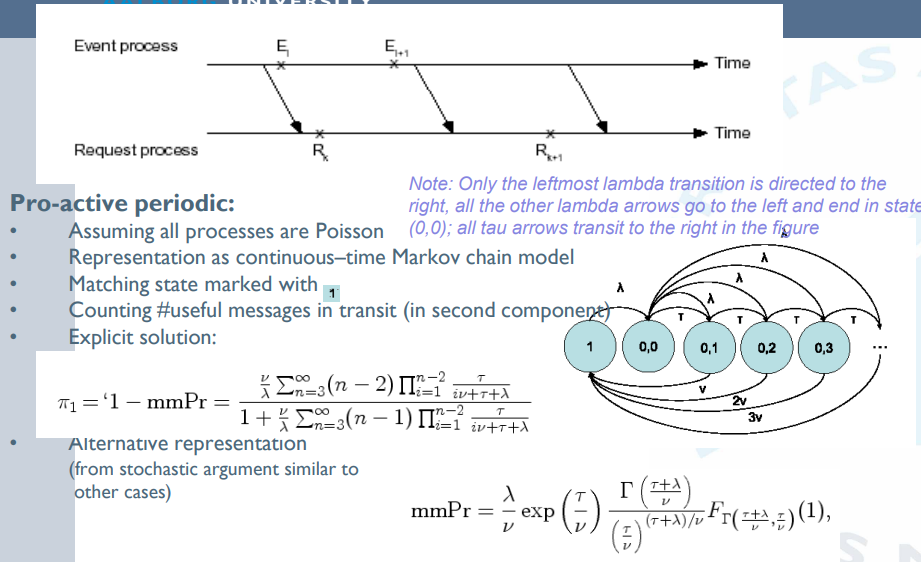
\includegraphics[width=\linewidth]{figures/Lecture7/periodicanal.png}
    \label{fig:placeholder}
\end{figure}

\section{Kendall's notation Again}

Queueing systems are described using \textbf{Kendall's notation}:
\[
  A \;/\; S \;/\; c \;/\; K
\]
 
\section*{The Four Fields}
 
\begin{center}
\begin{tabular}{clp{8cm}}
  \toprule
  \textbf{Position} & \textbf{Symbol} & \textbf{Meaning} \\
  \midrule
  1 & $A$ & Arrival process distribution \\
  2 & $S$ & Service time distribution \\
  3 & $c$ & Number of servers \\
  4 & $K$ & Buffer / system capacity (omitted $\Rightarrow$ infinite) \\
  \bottomrule
\end{tabular}
\end{center}
 
\section*{Distribution Letters}
 
\begin{center}
\begin{tabular}{cll}
  \toprule
  \textbf{Letter} & \textbf{Stands for} & \textbf{Meaning} \\
  \midrule
  $M$ & Memoryless (Markovian) & Poisson arrivals / Exponential service times \\
  $D$ & Deterministic           & Fixed, constant service time \\
  $G$ & General                 & Any arbitrary distribution \\
  \bottomrule
\end{tabular}
\end{center}
 
\section*{Reading the Examples from the Slides}
 
\begin{insightbox}
\textbf{M/M/$\infty$} --- Poisson arrivals, exponential service, infinitely
many servers, so no customer ever waits; they are served the instant they
arrive. Used for the \emph{incremental proactive} case: a message enters
service (network transit) the moment it is sent, and capacity is never
exhausted.
\end{insightbox}
 
\vspace{0.5em}
 
\begin{insightbox}
\textbf{M/D/1} --- Poisson arrivals, deterministic (fixed) service time,
1 server. Used for the \emph{reactive} case with a fixed network delay.
\end{insightbox}
 
\vspace{0.5em}
 
\begin{insightbox}
\textbf{M/G/1} --- Poisson arrivals, generally distributed service time,
1 server. The most general single-server case.
\end{insightbox}
 
\vspace{0.5em}
 
\begin{insightbox}
\textbf{E/D/1/1} --- A specific arrival process $E$, deterministic service,
1 server, and a \emph{buffer of size~1}. If a new message arrives while the
server is busy, it is dropped. Used for the \emph{proactive full-update}
case: only one message can be in the network at a time, modelling the
``last message still in transit'' logic for the mismatch probability.
\end{insightbox}
 
\vspace{0.5em}
 
\begin{insightbox}
\textbf{M/M/1/1} --- Poisson arrivals, exponential service, 1 server,
buffer of size~1. Any arriving customer finding the server busy is lost
(the system is \emph{loss} rather than \emph{delay}).
\end{insightbox}
 
\section*{The Buffer Field $K$}
 
When $K$ is omitted the buffer is assumed \textbf{infinite} by convention:
\[
  \text{M/M/1} \;\equiv\; \text{M/M/1/}\infty.
\]
Setting $K = c$ (equal to the number of servers) gives a \textbf{loss system}
--- there is no waiting room, so any customer that arrives when all servers are
busy is immediately turned away.





%============================================================
\section{Quantitative Results (Slide 10)}
% ============================================================
 
The figure on slide 10 plots $\mathrm{mmPr}$ against the downstream delay
rate $\nu$ for a Poisson event process with rate $\lambda = 1$.
\begin{figure}[H]
    \centering
    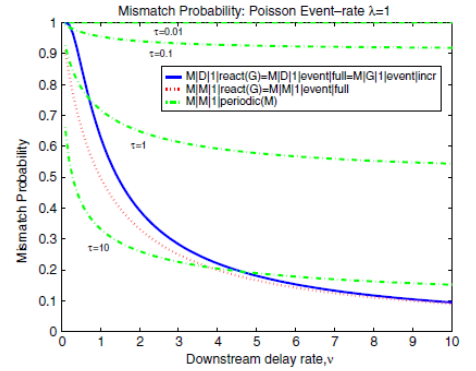
\includegraphics[width=0.75\linewidth]{figures/Lecture7/mmpr.png}
    \label{fig:placeholder}
\end{figure}
 
\subsection{Key Observations}
 
\begin{enumerate}[leftmargin=2em]
  \item \textbf{Blue curve} (deterministic delay, reactive and event-driven
        strategies):
        \[
          \mathrm{mmPr} = 1 - e^{-\lambda D},
        \]
        which decays smoothly as the network speeds up. The event-driven
        incremental strategy follows this same curve regardless of delay
        distribution.
 
  \item \textbf{Red curve} (exponential delay, reactive = event-driven full):
        \[
          \mathrm{mmPr} = \frac{\lambda}{\lambda + \nu},
        \]
        which is \emph{better} than the deterministic case --- a
        counter-intuitive result arising because lighter tails in the delay
        distribution are actually worse here.
 
  \item \textbf{Green dashed curves} (periodic, $\tau = 0.01, 0.1, 1, 10$):
        these do \emph{not} converge to zero as $\nu \to \infty$. They
        plateau at $\lambda/(\lambda+\tau)$, confirming the fundamental
        ceiling from the Markov chain analysis.
\end{enumerate}
 
\begin{insightbox}
\textbf{Practical takeaway:} for fast networks, event-driven or reactive
strategies are strictly superior to periodic ones. The periodic strategy
wastes the fast network because its accuracy is ultimately limited by the
update frequency, not the network speed.
\end{insightbox}
 
% ============================================================
\section{Controlled Offset in Periodic Communication (Slide 11)}
% ============================================================
 
Slide 11 introduces a practical refinement for the wind farm using
\textbf{deterministic periodic updates with a configurable offset} $T_o$.
\todo{still need to understand better but think later getting into it more}
\begin{figure}[H]
    \centering
    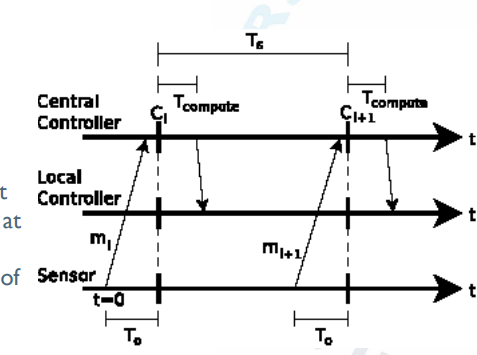
\includegraphics[width=0.5\linewidth]{figures/Lecture7/offsetcomputation.png}
    \label{fig:placeholder}
\end{figure}
 
\subsection{Timing Model}
 
\begin{itemize}[leftmargin=2em]
  \item $T_s = 150\,\text{ms}$ --- control period.
  \item $T_{\text{compute}} = 50\,\text{ms}$ --- time the controller needs to
        compute a new set-point after receiving data.
  \item $T_o$ --- offset: the sensor sends its measurement at $t = 0$, and
        the controller performs its computation at $C_i = T_o$.
  \item $C_i$ --- computation instant.
\end{itemize}
 
\subsection{The Trade-Off}
 
Choosing $T_o$ involves a fundamental tension:
 
\begin{center}
\begin{tabular}{lll}
  \toprule
  & \textbf{Small $T_o$} & \textbf{Large $T_o$} \\
  \midrule
  Delivery risk & High (message may not arrive) & Low \\
  Data age      & Low (fresh if it arrives)     & High (stale by use time) \\
  \bottomrule
\end{tabular}
\end{center}
 
There is an \textbf{optimal $T_o$} somewhere between these extremes. Finding
it analytically --- rather than by exhaustive simulation --- motivates the
data quality model developed in the second half of the lecture.

% ============================================================
\section*{Summary of Notation}
% ============================================================
 
\begin{center}
\begin{tabular}{cl}
  \toprule
  \textbf{Symbol} & \textbf{Meaning} \\
  \midrule
  $\lambda$ & Event rate (Poisson sensor value changes) \\
  $\mu$     & Request rate (controller polling) \\
  $\nu$     & Downstream delay rate (sensor $\to$ controller) \\
  $\tau$    & Update period rate (proactive periodic) \\
  $\mathrm{mmPr}$ & Mismatch probability \\
  $\mathcal{L}\{f_D\}(\lambda)$ & Laplace transform of delay PDF at $\lambda$ \\
  $T_s$     & Control period (150 ms) \\
  $T_o$     & Communication offset \\
  $T_{\text{compute}}$ & Controller computation time (50 ms) \\
  $C_i$     & $i$-th computation instant \\
  \bottomrule
\end{tabular}
\end{center}
\clearpage

\begin{center}
  {\LARGE\bfseries\color{aaublue}
    MM7 subsection Networks and Systems}\\[0.4em]
  {\large\color{accentgray}
    Topic Notes: Controller performance}\\[0.2em]
  {\large\bfseries Slides 13--15}\\[0.3em]
  {\small\color{accentgray}
    Hans-Peter Schwefel, Aalborg University}
\end{center}
% ============================================================
\section{Effect of Network Delay on Controller Performance (Slide 13)}
% ============================================================
 
\subsection{Scenario}
 
The setup holds the offset fixed at $T_o = 75\,\text{ms}$ while the mean
network delay from sensor to controller is gradually increased. The delay
follows a \textbf{shifted exponential distribution} --- meaning there is a
guaranteed minimum delay, with a random exponential component added on top.
\begin{figure}[H]
    \centering
    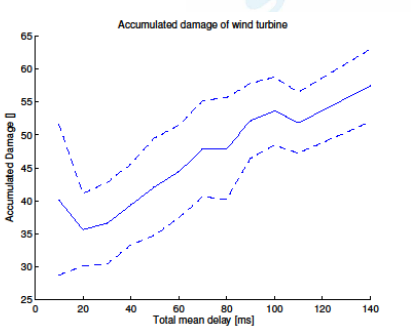
\includegraphics[width=0.6\linewidth]{figures/Lecture7/differentmeandelay.png}
    \label{fig:placeholder}
\end{figure} 
\subsection{Observation}
 
The simulation result is straightforward but important:
 
\begin{insightbox}
Once the mean network delay exceeds approximately $20\,\text{ms}$, accumulated
turbine damage rises steadily with increasing delay. The controller is
working with increasingly stale data, so its decisions progressively worsen.
\end{insightbox}
 
This confirms the intuitive expectation that network quality directly impacts
control performance --- but it also quantifies \emph{where} the threshold
lies. Below $20\,\text{ms}$, the system is relatively tolerant of delay
variation; beyond it, every additional millisecond of delay costs measurable
damage.
 
% ============================================================
\section{Effect of Offset on Controller Performance (Slide 14)}
% ============================================================
 
\subsection{Scenario}
 
Now the mean delay is fixed at $30\,\text{ms}$ (shifted exponential,
$1\,\text{ms}$ minimum) and the offset $T_o$ is varied between
$10\,\text{ms}$ and $150\,\text{ms}$.
 
\subsection{Observation}
 
The accumulated damage as a function of $T_o$ has a clear shape with a
distinct minimum:
 
\begin{itemize}[leftmargin=2em]
  \item Damage \textbf{decreases} as $T_o$ increases -- up to
        $T_o \approx 100\,\text{ms}$.
  \item Beyond $T_o = 100\,\text{ms}$, damage \textbf{rises again}.
\end{itemize}
 \begin{figure}[H]
     \centering
     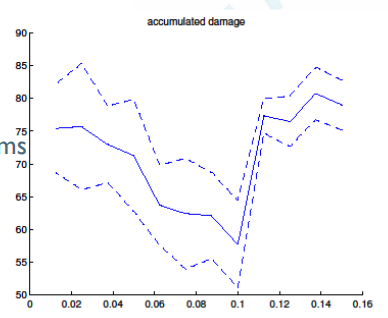
\includegraphics[width=0.6\linewidth]{figures/Lecture7/differentoffset.png}
     \label{fig:placeholder}
 \end{figure}
\subsection{Explanation of the Trade-Off}
 
This U-shaped behaviour reflects the fundamental tension introduced in
Slide~11:
 
\begin{center}
\begin{tabular}{lp{5.5cm}p{5.5cm}}
  \toprule
  & \textbf{Small $T_o$} & \textbf{Large $T_o$} \\
  \midrule
  Delivery & Message may not have arrived yet $\Rightarrow$ controller
             uses old data & Message reliably arrives in time \\[0.5em]
  Data age  & Fresh (if it arrives) & Stale by the time it is used \\[0.5em]
  Result    & Mismatch due to late delivery & Mismatch due to aged data \\
  \bottomrule
\end{tabular}
\end{center}
 
\vspace{0.5em}
 
At $T_o = 100\,\text{ms}$ the wind turbine begins receiving the
\textbf{previous} control period's set-point. Beyond this point the
controller is effectively operating one full cycle behind, causing damage
to climb steeply regardless of how fresh the sensor data is.
 
\begin{insightbox}
\textbf{Key result:} there exists an optimal offset $T_o^*$ that balances
delivery reliability against data freshness. For this scenario,
$T_o^* \approx 100\,\text{ms}$.
\end{insightbox}
 
% ============================================================
\section{Offset Optimisation (Slide 15)}
% ============================================================
 
\subsection{The Problem}
 
Slide~14 demonstrates that the choice of $T_o$ matters greatly, but finding
$T_o^*$ by running a full control simulation for every candidate value is
\textbf{very time consuming}. A smarter approach is needed.
 
\subsection{Two Approaches}
 
\subsubsection*{Baseline}
 
Pick $T_o$ uniformly at random from $[0,\, 150\,\text{ms}]$. This ignores
all knowledge of the delay distribution and unsurprisingly performs poorly.
 
\subsubsection*{Heuristic: $p$-th Percentile of the Delay Distribution}
 
Set the offset to the $p$-th percentile of the measured sensor-to-controller
delay distribution:
\[
  T_o = F_D^{-1}(p),
\]
where $F_D$ is the CDF of the delay. The reasoning is:
 
\begin{itemize}[leftmargin=2em]
  \item If $T_o = F_D^{-1}(p)$, then a fraction $p$ of all messages will
        have arrived by the time the controller computes.
  \item A higher $p$ gives more delivery reliability but at the cost of a
        larger --- and therefore staler --- offset.
  \item A lower $p$ keeps data fresh but risks messages not arriving in time.
\end{itemize}
 
\subsection{Results}
 
The bar chart on Slide~15 compares accumulated damage across five cases:
 
\begin{center}
\begin{tabular}{lp{9cm}}
  \toprule
  \textbf{Case} & \textbf{Observation} \\
  \midrule
  Baseline         & Highest damage; uninformed choice performs worst. \\
  Heuristic 99\%   & Very conservative $T_o$; data becomes too old. \\
  Heuristic 95\%   & Good performance; reliable delivery, acceptable age. \\
  Heuristic 90\%   & Best or near-best; sweet spot for this scenario. \\
  Heuristic 80\%   & Slightly worse; some messages still miss the deadline. \\
  \bottomrule
\end{tabular}
\end{center}
\begin{figure}[H]
    \centering
    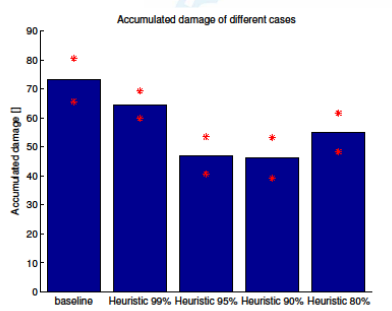
\includegraphics[width=0.7\linewidth]{figures/Lecture7/percentiledelayset.png}
    \label{fig:placeholder}
\end{figure}
\vspace{0.5em}
 
All heuristics significantly outperform the baseline. The middle percentiles
($p = 90\text{--}95\%$) perform best: $p = 99\%$ is overly conservative
(the offset grows so large that data ages too much), while $p = 80\%$ is
too aggressive (too many messages miss the deadline).
 
\subsection{Open Question}
 
\begin{insightbox}
\textbf{How should $p$ be chosen systematically?} The heuristic works well
given a ``good'' choice of $p$, but selecting $p$ still requires either
intuition or trial-and-error. This motivates the \textbf{data quality model}
developed from Slide~17 onwards: rather than optimising damage directly
via expensive simulation, the idea is to optimise the analytically tractable
mismatch probability $\mathrm{mmPr}$, which serves as a proxy for control
performance.
\end{insightbox}
\clearpage
\begin{center}
  {\LARGE\bfseries\color{aaublue}
    MM7 subsection Networks and Systems}\\[0.4em]
  {\large\color{accentgray}
    Topic Notes: Data quality model for wind-farm scenario}\\[0.2em]
  {\large\bfseries Slides 17--23}\\[0.3em]
  {\small\color{accentgray}
    Hans-Peter Schwefel, Aalborg University}
\end{center}
% 

% ============================================================
\section{Motivation: Why a Data Quality Model? (Slide 17)}
% ============================================================
 
Running full control simulations to find the optimal offset $T_o$ is
computationally expensive. Every candidate value of $T_o$ requires a
complete simulation of the wind turbine physics, the communication network,
and the control loop --- which can take a long time per run.
 
The key idea is to instead optimise a \textbf{simpler analytical proxy
metric} that can be evaluated quickly without simulation. This metric is
called the \textbf{mismatch probability} $\mathrm{mmPr}(\epsilon)$, defined
as:
\[
  \mathrm{mmPr}(\epsilon)
    := \Pr\!\bigl(|X_s(C_i) - X_C(C_i)| > \epsilon\bigr),
\]
where:
\begin{itemize}[leftmargin=2em]
  \item $X_s(C_i)$ is the \textbf{true sensor value} at computation
        instant $C_i$,
  \item $X_C(C_i)$ is the \textbf{controller's belief} about the sensor
        value at that same instant,
  \item $\epsilon$ is a tolerance threshold.
\end{itemize}
 
In plain terms: $\mathrm{mmPr}(\epsilon)$ is the probability that what the
controller \emph{thinks} the sensor reads differs from what the sensor
\emph{actually} reads by more than $\epsilon$. A high $\mathrm{mmPr}$ means
the controller is frequently working with significantly outdated or incorrect
data.
 
Two questions motivate the rest of the section:
 
\begin{enumerate}[leftmargin=2em]
  \item Is minimising $\mathrm{mmPr}$ actually equivalent to minimising
        turbine damage (control performance)?
  \item Can $\mathrm{mmPr}$ be computed from a simple analytical model,
        avoiding simulation entirely?
\end{enumerate}
 
\begin{insightbox}
If both answers are yes, we can find the optimal $T_o$ cheaply by minimising
$\mathrm{mmPr}$ analytically, and trust that this also minimises damage.
\end{insightbox}
 
% ============================================================
\section{Inspecting the Sensor Data (Slide 18)}
% ============================================================
 
Before building a model, the actual sensor behaviour is examined. A control
simulation is run under \emph{ideal} communication (no delay, no loss), and
all sensor measurements are recorded. Plotting this trace reveals two
distinct types of behaviour:
 
\begin{itemize}[leftmargin=2em]
  \item \textbf{Smooth drift} between controller actuations --- the sensor
        value evolves gradually as the turbine responds to wind.
  \item \textbf{Sudden sharp jumps} at actuation instants --- when the
        controller issues a new set-point, the turbine state changes abruptly,
        which immediately shows up in the sensor readings as a large spike in
        the difference time series (the downward peaks visible in the bottom
        plot of slide 18).
\end{itemize}
\begin{figure}[H]
    \centering
    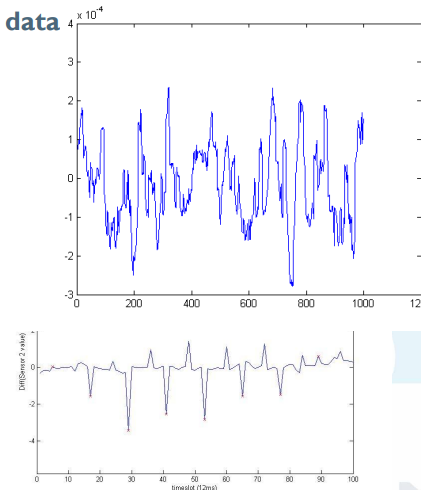
\includegraphics[width=0.7\linewidth]{figures/Lecture7/tworegime.png}
    \label{fig:placeholder}
\end{figure}
 
This two-regime structure is important: the sensor does not evolve uniformly
over time. Actuations introduce a qualitatively different kind of change that
a single statistical model would struggle to capture well. This motivates
splitting the model explicitly into two parts.
 
% ============================================================
\section{Markov Chain Model of the Sensor (Slide 19)}
% ============================================================
 
\subsection{What Are We Actually Modelling?}
 
The goal is to model the \textbf{sensor value itself} as a stochastic
process, so that we can compute probabilities about how much it may have
changed over a given time interval. The sensor produces a continuous physical
value (e.g.\ torque in Nm), but working with continuous distributions is
complex. Instead, the value space is \textbf{discretised into $N$ equal
bins} --- so rather than tracking the exact value, we track which bin the
value falls into. Each bin is a \textbf{state}, giving a state space of size
$N$.
 
The sensor's evolution is then modelled as a \textbf{discrete-time Markov
chain}: at each timestep, the system moves from one state to another
according to a matrix of transition probabilities. Entry $(j, k)$ of the
transition matrix gives the probability of moving from state $j$ to state
$k$ in one step. These probabilities are estimated \emph{empirically} from
the recorded sensor trace.
 
Once we have this model, the central question becomes:
 
\begin{insightbox}
Given that the sensor was in state $k$ at time $C_i - T_o$ (when the
message was sent), what is the probability it is \emph{still} in state $k$
at time $C_i$ (when the controller uses the data)? If it stayed in the same
state, the controller has correct information. If it moved, that is a
mismatch.
\end{insightbox}
 
The probability of being in a particular state after $n$ steps is given by
the $n$-th power of the transition matrix. This is the key computation that
makes the whole approach analytically tractable.
 
\subsection{Approach I: Single Transition Matrix}
 
The simplest approach treats the entire sensor trace uniformly. A single
$N \times N$ transition matrix $P_0$ is estimated from all timestep
transitions in the recorded data, regardless of whether they occur during
normal operation or at actuation instants.
 
\[
  P_0 \;\in\; \mathbb{R}^{N \times N},
  \quad
  (P_0)_{jk} = \Pr(\text{state } k \text{ at step } t{+}1
                    \mid \text{state } j \text{ at step } t).
\]
 
This is straightforward to implement and requires only one matrix. However,
it conflates two qualitatively different types of transitions --- the smooth
drift and the actuation jumps --- into a single average. This averaging can
reduce accuracy, particularly around actuation instants where the sensor
behaviour is very different.
 
\subsection{Approach II: Separate Matrices for Each Regime}
 
The refined approach explicitly captures the two-regime structure observed
in slide 18. Two separate $N \times N$ transition matrices are estimated:
 
\begin{itemize}[leftmargin=2em]
  \item \textbf{Matrix $P$} (normal evolution) --- estimated from all
        transitions that occur \emph{between} actuation instants, where the
        sensor drifts smoothly. This matrix has entries close to the identity
        for small $N$, reflecting that the sensor tends to stay in the same
        bin or move to a neighbouring one.
 
  \item \textbf{Matrix $C$} (actuation transitions) --- estimated only from
        the transitions that occur \emph{at} actuation instants, where the
        controller fires a new command and the sensor jumps abruptly. This
        matrix will have much more spread, reflecting that an actuation can
        push the sensor into a very different state.
\end{itemize}
 
Crucially, $P$ and $C$ are \textbf{not two states} --- they are two full
$N \times N$ matrices defined over the same $N$ sensor-value states. The
distinction is about \emph{what kind of timestep} is occurring, not about
which state the sensor is in.
 
To compute the probability of being in state $k$ after a sequence of
timesteps that includes both normal steps and actuation steps, the
appropriate matrices are multiplied together in sequence. For example, over
one control period of length $T_s$ containing one actuation:
\[
  \text{(combined transition)} = P^{n_1} \cdot C \cdot P^{n_2},
\]
where $n_1$ and $n_2$ are the number of normal timesteps before and after
the actuation respectively.
 
\begin{insightbox}
\textbf{Why does this matter?} If the data used by the controller was
captured \emph{before} an actuation and the controller computes \emph{after}
it, the sensor state may have jumped significantly. Approach II correctly
accounts for this jump via matrix $C$, whereas Approach I would only see a
smoothed-out average transition --- underestimating the risk of mismatch
around actuation instants.
\end{insightbox}
 
% ============================================================
\section{Computing mmPr from the Markov Model (Slide 20)}
% ============================================================
 
With the Markov model in place, $\mathrm{mmPr}$ can be computed analytically.
The formula accounts for two cases depending on whether the most recent
update message arrived before the controller's computation instant $C_i$.
 
Let:
\begin{itemize}[leftmargin=2em]
  \item $F_D(t)$ be the CDF of the network delay distribution,
  \item $T_o$ be the offset (time from message send to computation),
  \item $T_c = T_s - T_o$ be the remaining time in the control period,
  \item $\pi_u(k)$ be the stationary probability of state $k$ under the
        Markov chain,
  \item $\Pr(\text{state } k \text{ at } C_i \mid \text{state } k \text{ at }
        C_i - \Delta t)$ be the $(k,k)$ entry of the appropriate matrix
        power, giving the probability of remaining in state $k$ over an
        interval $\Delta t$.
\end{itemize}
 
The full expression for the matching probability is:
 
\begin{align}
  1 - \mathrm{mmPr}
  &= F_D(T_o) \sum_{k=1}^{N} \pi_u(k) \cdot
     \Pr\!\bigl(\text{state } k \text{ at } C_i
               \mid \text{state } k \text{ at } C_i - T_o\bigr)
  \notag \\
  &\quad + \bigl(1 - F_D(T_o)\bigr)\, F_D(T_o + T_c)
     \sum_{k=1}^{N} \pi_u(k) \cdot
     \Pr\!\bigl(\text{state } k \text{ at } C_i
               \mid \text{state } k \text{ at } C_i - T_o - T_c\bigr).
\end{align}
 
\subsection{Unpacking the Two Terms}
 
\subsubsection*{Term 1: latest message arrives in time}
 
$F_D(T_o)$ is the probability that the message sent at offset $T_o$ before
$C_i$ has arrived by $C_i$. If it has, the controller holds data that is
$T_o$ old. The Markov chain then gives the probability that the sensor is
still in the same state $k$ after $T_o$ timesteps --- which is the $(k,k)$
diagonal entry of the appropriate matrix power. Summing over all states $k$,
weighted by the stationary distribution $\pi_u(k)$, gives the overall
probability of a match in this case.
 
\subsubsection*{Term 2: latest message misses, previous one arrives}
 
$(1 - F_D(T_o))$ is the probability the latest message has \emph{not} yet
arrived. In that case the controller falls back on the message from the
\emph{previous} control period, which was sent $T_o + T_c$ before $C_i$.
$F_D(T_o + T_c)$ is the probability that this older message did arrive. The
Markov chain now needs to span a longer interval $T_o + T_c$, meaning more
matrix steps and a lower probability of the sensor still being in the same
state.
 
\begin{insightbox}
\textbf{Key insight:} the entire computation reduces to matrix
multiplications --- no simulation required. The $(k,k)$ diagonal entries of
$P^n$ (or the combined $P^{n_1} C\, P^{n_2}$ product in Approach II) give
the stay-probability directly. The optimal $T_o$ is then found by minimising
$\mathrm{mmPr}$ over $T_o$, which is a fast one-dimensional search.
\end{insightbox}
 
% ============================================================
\section{Results from the Markov Model (Slide 21)}
% ============================================================
 
The model is applied to sensor 3 data using Approach II, with the number of
discretisation states $N$ varying from 2 to 12. The plot on slide 21 shows
$\mathrm{mmPr}$ as a function of $T_o$ for each value of $N$.
 \begin{figure}[H]
     \centering
     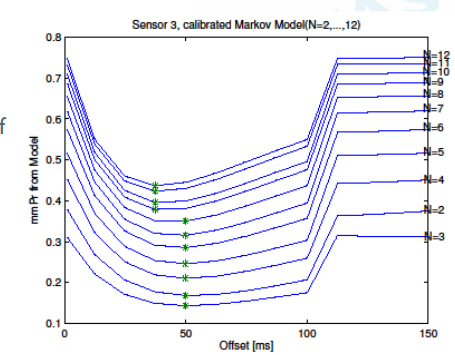
\includegraphics[width=0.6\linewidth]{figures/Lecture7/binsamountmmpr.png}
     \label{fig:placeholder}
 \end{figure}
Two observations stand out:
 
\begin{itemize}[leftmargin=2em]
  \item \textbf{All curves show a clear minimum} --- confirming that the
        model correctly captures the trade-off between delivery reliability
        and data freshness identified in slide 14.
 
  \item \textbf{The location of the minimum shifts slightly with $N$:}
        \begin{itemize}
          \item For $N \leq 8$: minimum at $T_o = 50\,\text{ms}$.
          \item For $8 < N \leq 12$: minimum at $T_o = 37.5\,\text{ms}$.
        \end{itemize}
        Finer discretisation captures more detail about how quickly the
        sensor state changes between bins, suggesting that with higher
        resolution the sensor appears to evolve faster --- making a slightly
        shorter offset optimal.
\end{itemize}
 
% ============================================================
\section{Validation: Mismatch Metric (Slide 22)}
% ============================================================
 
The $\mathrm{mmPr}$ predicted by the Markov model is compared directly
against $\mathrm{mmPr}$ measured from the full control simulation. The
results show:
\begin{figure}[H]
    \centering
    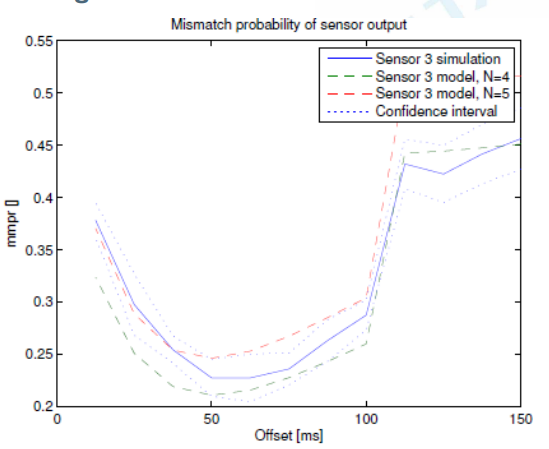
\includegraphics[width=0.65\linewidth]{figures/Lecture7/karmovvssim.png}
    \label{fig:placeholder}
\end{figure}
 
\begin{itemize}[leftmargin=2em]
  \item \textbf{Qualitatively good match} --- the predicted and simulated
        curves follow the same shape across the full range of $T_o$.
  \item \textbf{The minimum occurs at the same offset} --- both the model
        and the simulation agree that $T_o = 50\,\text{ms}$ is optimal, for
        $N = 4$ states in the Markov model.
\end{itemize}
 
Notably, $N = 4$ is a very coarse discretisation --- the sensor value space
is divided into only 4 bins. The fact that this already reproduces the
correct optimum demonstrates that the Markov model does not need to be
highly detailed to be useful as an optimisation tool.
 
% ============================================================
\section{Validation: Control Performance (Slide 23)}
% ============================================================
 
The final validation step checks whether minimising $\mathrm{mmPr}$ actually
corresponds to minimising turbine damage.
prediction.

\begin{insightbox}
\textbf{This kind of validates the central hypothesis from slide 17:} So the honest reading of slide 23 is actually more nuanced — the mmPr minimum and the damage minimum do **not** perfectly coincide. The Markov model predicts $T_o \approx 50\,\text{ms}$
as optimal, but actual damage is minimised somewhere around $
80–90\,\text{ms}$. This is an important distinction because it means the answer to the first question from slide 17 — *is optimising mmPr equivalent to optimising control performance?* — is **only approximately yes**. The model gets you in the right ballpark but is not perfectly aligned with damage minimisation.
\end{insightbox}
\begin{figure}[H]
    \centering
    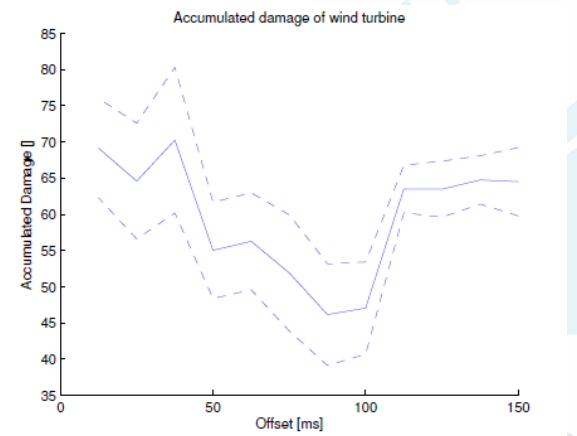
\includegraphics[width=0.6\linewidth]{figures/Lecture7/damageoffset.png}
    \label{fig:placeholder}
\end{figure}

\todo[inline]{Have not looked at this yet can be done if interested but no part of exammen
Wind-farm scenario using OTS (off-theshelf) communication technologies–not
part of exam
}